\documentclass[./../main.tex]{subfiles}
\graphicspath{{img/}}

\begin{document}
    \problempts{5}

    \section{Campo de desplazamientos}

    Graficar el campo de desplazamientos de una barra prismática bajo su propio peso dado por:

    \begin{align*}
        u &= \dfrac{-\nu\rho gxz}{E},\\
        v &= \dfrac{-\nu\rho gyz}{E},\\
        w &= \dfrac{\rho g}{2E}\Bigl[z^{2} + \nu(x^{2} + y^{2}) - L^{2}\Bigr]
    \end{align*}

    con \(\nu\) el coeficiente de Poisson, \(E\) el módulo de Young, \(g\) la aceleración debida al campo gravitacional y \(L\) la longitud del material.

    El campo de desplazamientos para este problema se ve como se muestra en la \cref{fig:displacement-field}

    \begin{figure}[htb]
        \centering
        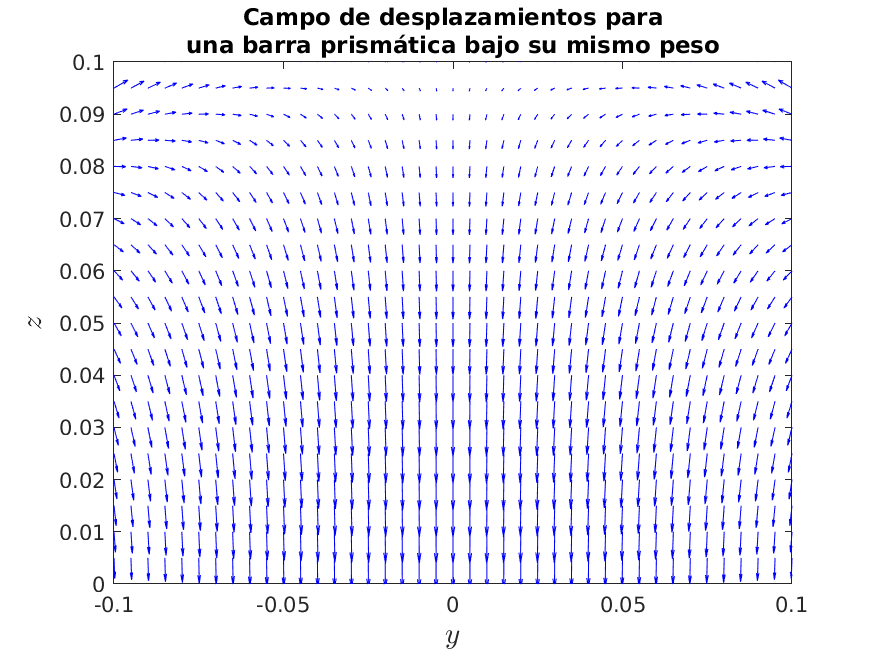
\includegraphics[scale=0.75]{campodesplazamientos}
        \caption{Campo de desplazamientos de una barra prismática bajo su propio peso.}
        \label{fig:displacement-field}
    \end{figure}
\end{document}